\section{paleoTS}

\subsection{all (continental and
	insular)}\label{all-continental-and-insularAP}

\begin{longtable}[]{@{}rrrr@{}}
	\caption{paleoTS object, all data}
	\label{tab:pTSall}\tabularnewline
	\toprule
	tt & mm & vv & nn\tabularnewline
	\midrule
	\endfirsthead
	\toprule
	tt & mm & vv & nn\tabularnewline
	\midrule
	\endhead
	0.0000005 & 401.9641 & 102306.64 & 4\tabularnewline
	0.0058500 & 314.1859 & 42607.58 & 18\tabularnewline
	0.0688500 & 506.3265 & 64620.11 & 8\tabularnewline
	0.4535000 & 516.4053 & 155241.85 & 7\tabularnewline
	1.2935000 & 593.8669 & 147507.20 & 12\tabularnewline
	2.1970000 & 971.8850 & 580540.76 & 8\tabularnewline
	3.0940000 & 658.0826 & 271043.73 & 9\tabularnewline
	4.4660000 & 785.0792 & 187937.61 & 8\tabularnewline
	6.2890000 & 1141.9375 & 584378.85 & 4\tabularnewline
	9.4270000 & 703.9570 & 195766.19 & 9\tabularnewline
	12.7140000 & 628.3020 & 285258.36 & 6\tabularnewline
	14.8950000 & 687.9619 & 169914.58 & 7\tabularnewline
	19.5000000 & 441.5420 & 78467.65 & 9\tabularnewline
	\bottomrule
\end{longtable}


\FloatBarrier

\subsection{continental (excluding insular
	species)}\label{continental-excluding-insular-speciesAP}



\begin{longtable}[H]{@{}rrrr@{}}
	\caption{paleoTS object, continental}
	\label{tab:pTSC}\tabularnewline
	\toprule
	tt & mm & vv & nn\tabularnewline
	\midrule
	\endfirsthead
	\toprule
	tt & mm & vv & nn\tabularnewline
	\midrule
	\endhead
	0.0000005 & 233.1680 & 8331.753 & 3\tabularnewline
	0.0058500 & 241.7917 & 13004.928 & 15\tabularnewline
	0.0688500 & 397.4606 & 50619.392 & 6\tabularnewline
	0.4535000 & 416.9341 & 200982.124 & 5\tabularnewline
	1.2935000 & 346.8484 & 66240.066 & 7\tabularnewline
	2.1970000 & 1103.1067 & 595507.933 & 7\tabularnewline
	3.0940000 & 725.4156 & 414253.291 & 6\tabularnewline
	4.4660000 & 771.3833 & 259173.082 & 6\tabularnewline
	6.2890000 & 1054.4375 & 531455.932 & 4\tabularnewline
	9.4270000 & 703.9570 & 195766.185 & 9\tabularnewline
	12.7140000 & 628.3020 & 285258.362 & 6\tabularnewline
	14.8950000 & 687.9619 & 169914.577 & 7\tabularnewline
	19.5000000 & 441.5420 & 78467.646 & 9\tabularnewline
	\bottomrule
\end{longtable}


\FloatBarrier

\subsection{insular (excluding
	continental)}\label{insular-excluding-continentalAP}


\begin{longtable}[]{@{}rrrr@{}}
	\caption{paleoTS object, insular}
	\label{tab:pTSI}\tabularnewline
	\toprule
	tt & mm & vv & nn\tabularnewline
	\midrule
	\endfirsthead
	\toprule
	tt & mm & vv & nn\tabularnewline
	\midrule
	\endhead
	0.0000005 & 860.9268 & 0.00 & 1\tabularnewline
	0.0058500 & 379.5354 & 68570.44 & 12\tabularnewline
	0.0688500 & 727.5938 & 14997.58 & 4\tabularnewline
	0.4535000 & 748.8333 & 142649.08 & 3\tabularnewline
	1.2935000 & 829.6744 & 112964.44 & 6\tabularnewline
	2.1970000 & 1178.3333 & 821158.33 & 3\tabularnewline
	3.0940000 & 449.4375 & 27058.77 & 4\tabularnewline
	4.4660000 & 826.1667 & 15196.06 & 2\tabularnewline
	6.2890000 & 1850.0000 & 0.00 & 1\tabularnewline
	\bottomrule
\end{longtable}


\FloatBarrier

\subsubsection{Europe, genera}\label{europe-genera}


\begin{longtable}[]{@{}rrrr@{}}
	\caption{paleoTS object, Europe}
	\label{tab:pTSEu}\tabularnewline
	\toprule
	mm & nn & vv & tt\tabularnewline
	\midrule
	\endfirsthead
	\toprule
	mm & nn & vv & tt\tabularnewline
	\midrule
	\endhead
	148.8559 & 2 & 3338.406 & 0.00585\tabularnewline
	616.6667 & 3 & 138802.333 & 0.06885\tabularnewline
	377.8167 & 3 & 89203.953 & 0.45350\tabularnewline
	697.3717 & 5 & 218431.974 & 1.29350\tabularnewline
	895.0000 & 2 & 1110050.000 & 2.19700\tabularnewline
	453.3333 & 3 & 39433.333 & 3.09400\tabularnewline
	1215.8667 & 5 & 159317.256 & 4.46600\tabularnewline
	838.3750 & 2 & 875495.281 & 6.28900\tabularnewline
	800.0508 & 6 & 263434.389 & 9.42700\tabularnewline
	653.9625 & 5 & 351634.528 & 12.71400\tabularnewline
	772.0000 & 5 & 223154.375 & 14.89500\tabularnewline
	533.8533 & 5 & 183706.682 & 19.50000\tabularnewline
	\bottomrule
\end{longtable}


\FloatBarrier





\subsubsection{Europe, genera, continental}\label{europe-genera-continental}

\begin{longtable}[]{@{}rrrr@{}}
	\caption{paleoTs object, Europe, continental}
	\label{tab:pTSEuC}\tabularnewline
	\toprule
	mm & nn & vv & tt\tabularnewline
	\midrule
	\endfirsthead
	\toprule
	mm & nn & vv & tt\tabularnewline
	\midrule
	\endhead
	149.5381 & 2 & 3450.8267 & 0.00585\tabularnewline
	187.0000 & 1 & 0.0000 & 0.06885\tabularnewline
	205.4750 & 2 & 198.0050 & 0.45350\tabularnewline
	204.9292 & 2 & 23.1767 & 1.29350\tabularnewline
	1420.0000 & 1 & 0.0000 & 2.19700\tabularnewline
	232.5000 & 1 & 0.0000 & 3.09400\tabularnewline
	1475.6667 & 3 & 57926.3333 & 4.46600\tabularnewline
	663.3750 & 2 & 473607.7812 & 6.28900\tabularnewline
	800.0508 & 6 & 263434.3893 & 9.42700\tabularnewline
	653.9625 & 5 & 351634.5281 & 12.71400\tabularnewline
	772.0000 & 5 & 223154.3750 & 14.89500\tabularnewline
	533.8533 & 5 & 183706.6821 & 19.50000\tabularnewline
	\bottomrule
\end{longtable}

\begin{figure}[H]
	\centering
	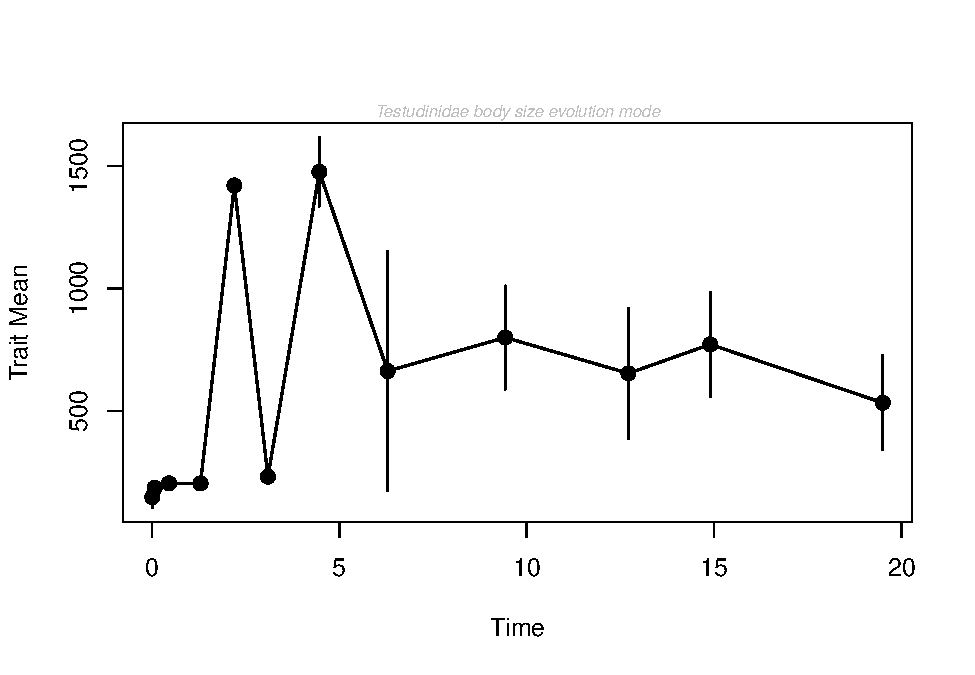
\includegraphics{MA_JJ_files/figure-latex/pTSEuC-1.pdf}
	\caption{paleoTS, genera, Europe, continental}
	\label{fig:pTSEuC}
\end{figure}

\begin{longtable}[]{@{}lrrrr@{}}
	\caption{Model-fitting results for testudinidae, genera, Europe,
		continental}
	\label{tab:pTSEuCEM}\tabularnewline
	\toprule
	& logL & K & AICc & Akaike.wt\tabularnewline
	\midrule
	\endfirsthead
	\toprule
	& logL & K & AICc & Akaike.wt\tabularnewline
	\midrule
	\endhead
	GRW & -87.93137 & 2 & 181.3627 & 0.009\tabularnewline
	URW & -92.56882 & 1 & 187.5821 & 0.000\tabularnewline
	Stasis & -83.21073 & 2 & 171.9215 & 0.991\tabularnewline
	\bottomrule
\end{longtable}


\FloatBarrier

%__________________________________________________________________________


\subsubsection{Europe, genera,
	insular}\label{europe-genera-insular}

\begin{longtable}[]{@{}rrrr@{}}
	\caption{paleoTs object, Europe, insular}
	\label{tab:pTSEuI}\tabularnewline
	\toprule
	mm & nn & vv & tt\tabularnewline
	\midrule
	\endfirsthead
	\toprule
	mm & nn & vv & tt\tabularnewline
	\midrule
	\endhead
	187.5077 & 1 & 0.00 & 0.00585\tabularnewline
	831.5000 & 2 & 684.50 & 0.06885\tabularnewline
	722.5000 & 1 & 0.00 & 0.45350\tabularnewline
	835.0833 & 4 & 168423.36 & 1.29350\tabularnewline
	1005.0000 & 2 & 1462050.00 & 2.19700\tabularnewline
	451.6667 & 3 & 40558.33 & 3.09400\tabularnewline
	826.1667 & 2 & 15196.06 & 4.46600\tabularnewline
	1850.0000 & 1 & 0.00 & 6.28900\tabularnewline
	\bottomrule
\end{longtable}

\begin{figure}[H]
	\centering
	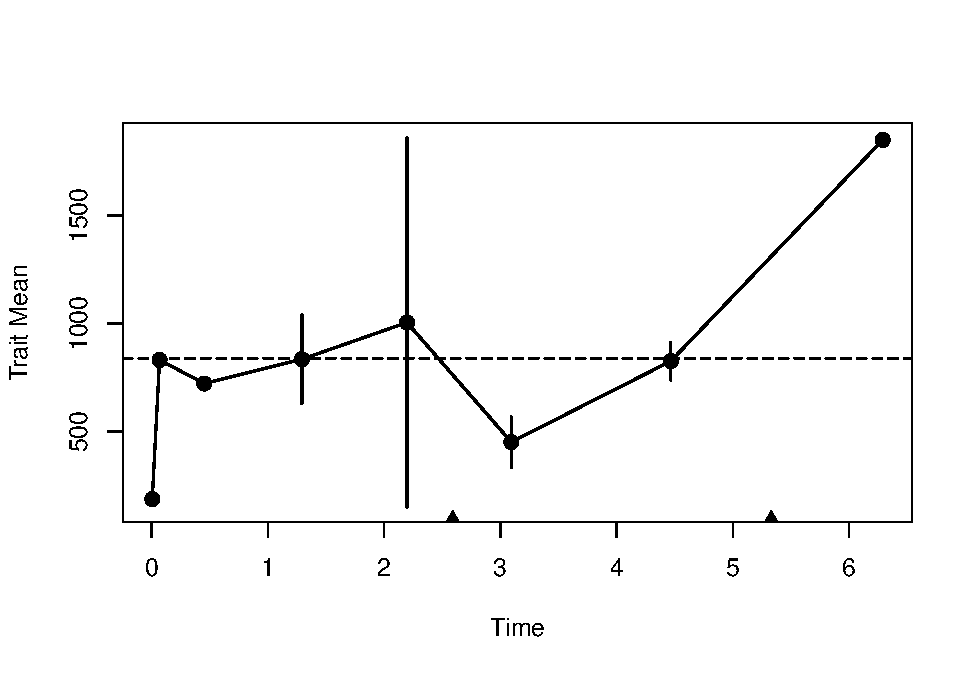
\includegraphics{MA_JJ_files/figure-latex/pTSEuI-1.pdf}
	\caption{paleoTS, genera, Europe, insular}
	\label{fig:pTSEuI}
\end{figure}

\begin{longtable}[]{@{}lrrrr@{}}
	\caption{Model-fitting results for testudinidae, genera, Europe,
		insular}
	\label{tab:pTSEuIEM}\tabularnewline
	\toprule
	& logL & K & AICc & Akaike.wt\tabularnewline
	\midrule
	\endfirsthead
	\toprule
	& logL & K & AICc & Akaike.wt\tabularnewline
	\midrule
	\endhead
	GRW & -67.12192 & 2 & 141.2438 & 0.000\tabularnewline
	URW & -57.51634 & 1 & 117.8327 & 0.074\tabularnewline
	Stasis & -52.89638 & 2 & 112.7928 & 0.926\tabularnewline
	\bottomrule
\end{longtable}

\FloatBarrier
%__________________________________________________________________________

\subsubsection{Eurasia,	genera}\label{eurasia-genera}


\begin{longtable}[]{@{}rrrr@{}}
	\caption{paleoTS object, Eurasia}
	\label{tab:pTSEs}\tabularnewline
	\toprule
	tt & mm & vv & nn\tabularnewline
	\midrule
	\endfirsthead
	\toprule
	tt & mm & vv & nn\tabularnewline
	\midrule
	\endhead
	0.0000005 & 137.2637 & 0.000 & 1\tabularnewline
	0.0058500 & 236.8217 & 9760.467 & 5\tabularnewline
	0.0688500 & 530.0000 & 122579.333 & 4\tabularnewline
	0.4535000 & 377.8167 & 89203.953 & 3\tabularnewline
	1.2935000 & 777.5579 & 162641.142 & 7\tabularnewline
	2.1970000 & 909.6667 & 562217.222 & 5\tabularnewline
	3.0940000 & 892.0000 & 381770.000 & 5\tabularnewline
	4.4660000 & 1048.0556 & 296417.219 & 6\tabularnewline
	6.2890000 & 1208.9167 & 849651.021 & 3\tabularnewline
	9.4270000 & 800.0508 & 263434.389 & 6\tabularnewline
	12.7140000 & 653.9625 & 351634.528 & 5\tabularnewline
	14.8950000 & 772.0000 & 223154.375 & 5\tabularnewline
	19.5000000 & 513.8533 & 162399.349 & 5\tabularnewline
	\bottomrule
\end{longtable}




\subsubsection{Eurasia, genera,
	continental}\label{eurasiagenera-continental}

\begin{longtable}[]{@{}rrrr@{}}
	\caption{paleoTS object, Eurasia, continental}
	\label{tab:pTSEsC}\tabularnewline
	\toprule
	tt & mm & vv & nn\tabularnewline
	\midrule
	\endfirsthead
	\toprule
	tt & mm & vv & nn\tabularnewline
	\midrule
	\endhead
	0.0000005 & 137.2637 & 0.000 & 1\tabularnewline
	0.0058500 & 238.0120 & 9654.865 & 5\tabularnewline
	0.0688500 & 228.5000 & 3444.500 & 2\tabularnewline
	0.4535000 & 205.4750 & 198.005 & 2\tabularnewline
	1.2935000 & 595.5388 & 191487.404 & 4\tabularnewline
	2.1970000 & 1044.5833 & 442006.250 & 4\tabularnewline
	3.0940000 & 1110.8333 & 581102.083 & 3\tabularnewline
	4.4660000 & 1159.0000 & 439728.667 & 4\tabularnewline
	6.2890000 & 1092.2500 & 788605.188 & 3\tabularnewline
	9.4270000 & 800.0508 & 263434.389 & 6\tabularnewline
	12.7140000 & 653.9625 & 351634.528 & 5\tabularnewline
	14.8950000 & 772.0000 & 223154.375 & 5\tabularnewline
	19.5000000 & 513.8533 & 162399.349 & 5\tabularnewline
	\bottomrule
\end{longtable}

\begin{figure}[H]
	\centering
	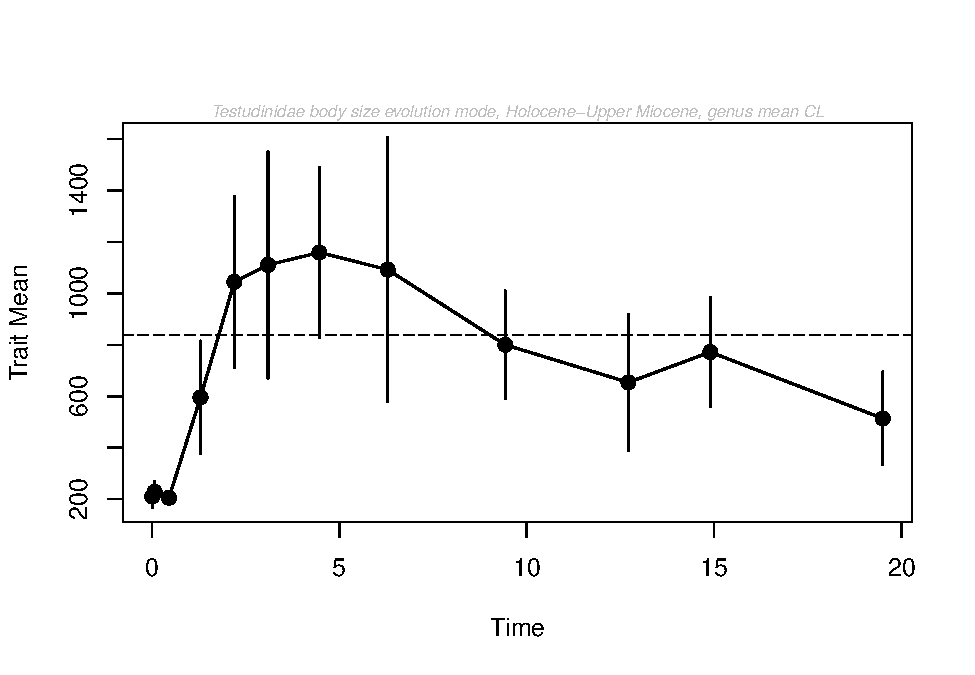
\includegraphics{MA_JJ_files/figure-latex/pTSEsC-1.pdf}
	\caption{paleoTS, genera, Eurasia, continental}
	\label{fig:pTSEsC}
\end{figure}

\begin{longtable}[]{@{}lrrrr@{}}
	\caption{Model-fitting results for testudinidae, genera, Eurasia,
		continental}
	\label{tab:pTSEsCEM}\tabularnewline
	\toprule
	& logL & K & AICc & Akaike.wt\tabularnewline
	\midrule
	\endfirsthead
	\toprule
	& logL & K & AICc & Akaike.wt\tabularnewline
	\midrule
	\endhead
	GRW & -82.20698 & 2 & 169.7473 & 0.222\tabularnewline
	URW & -82.42344 & 1 & 167.2469 & 0.776\tabularnewline
	Stasis & -87.19538 & 2 & 179.7241 & 0.002\tabularnewline
	\bottomrule
\end{longtable}


\FloatBarrier
%__________________________________________________________________________

\subsubsection{Eurasia, genera,
	insular}\label{eurasiagenera-insular}

\begin{longtable}[]{@{}rrrr@{}}
	\caption{paleoTS object, Eurasia, insular}
	\label{tab:pTSEsI}\tabularnewline
	\toprule
	tt & mm & vv & nn\tabularnewline
	\midrule
	\endfirsthead
	\toprule
	tt & mm & vv & nn\tabularnewline
	\midrule
	\endhead
	0.0000005 & 137.2637 & 0.000 & 1\tabularnewline
	0.0058500 & 271.4596 & 5668.485 & 4\tabularnewline
	0.0688500 & 644.3333 & 105436.333 & 3\tabularnewline
	0.4535000 & 722.5000 & 0.000 & 1\tabularnewline
	1.2935000 & 882.0356 & 105684.077 & 6\tabularnewline
	2.1970000 & 953.6667 & 652233.889 & 5\tabularnewline
	3.0940000 & 891.0000 & 383430.000 & 5\tabularnewline
	4.4660000 & 620.4444 & 134562.926 & 3\tabularnewline
	6.2890000 & 1900.0000 & 5000.000 & 2\tabularnewline
	19.5000000 & 800.0000 & 0.000 & 1\tabularnewline
	\bottomrule
\end{longtable}

\newpage

\begin{figure}[H]
	\centering
	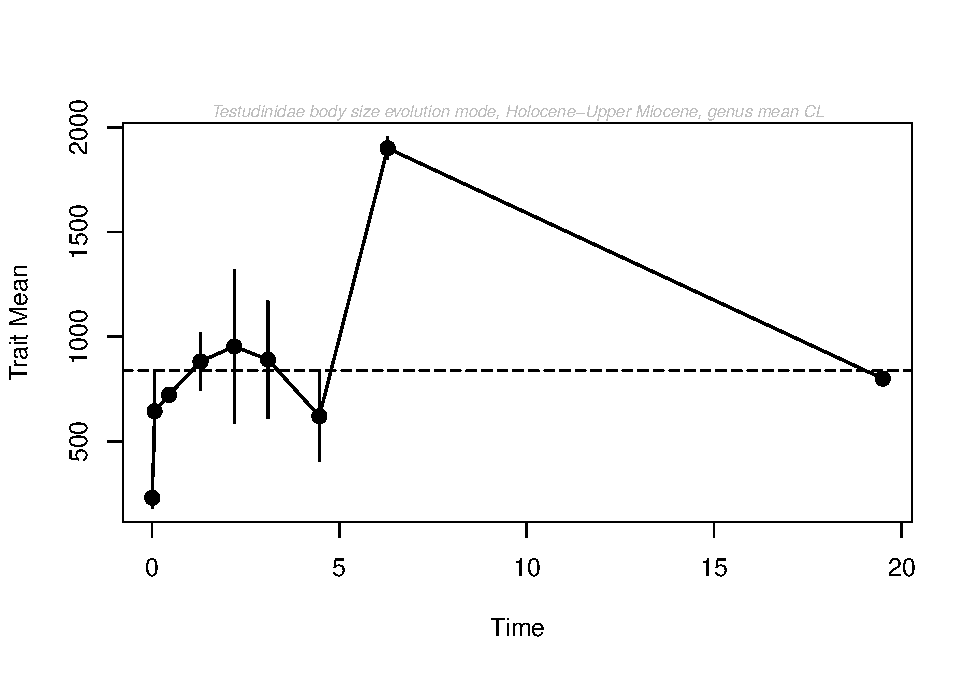
\includegraphics{MA_JJ_files/figure-latex/pTSEsI-1.pdf}
	\caption{paleoTS, genera, Eurasia, insular}
	\label{fig:pTSEsI}
\end{figure}

\begin{longtable}[]{@{}lrrrr@{}}
	\caption{Model-fitting results for testudinidae, genera, Eurasia,
		insular}
	\label{tab:pTSEsIEM}\tabularnewline
	\toprule
	& logL & K & AICc & Akaike.wt\tabularnewline
	\midrule
	\endfirsthead
	\toprule
	& logL & K & AICc & Akaike.wt\tabularnewline
	\midrule
	\endhead
	GRW & -69.56419 & 2 & 145.1284 & 0.193\tabularnewline
	URW & -71.67437 & 1 & 145.9202 & 0.130\tabularnewline
	Stasis & -68.31026 & 2 & 142.6205 & 0.677\tabularnewline
	\bottomrule
\end{longtable}


\FloatBarrier






